\chapter{东亚下方CMB结构}

本章主要利用国家测震台网的PKiKP/PcP振幅比和走时残差数据,简要分析中国下方CMB的结构变化. 首先,前一节通
过振幅比和走时残差分析,研究CMB的中型尺度范围的变化;后一小结通过对比相同台站对两个不同时间,震级不同,但位置和震源深度都很接近的两个地震的PKiKP和PcP观测结果,讨论引起振幅比观测波动的因素. 

\section{振幅比和走时残差分析}

第二章中提到,利用国家测震台网,本研究发现了两个产生超过500个单道可识别的PKiKP信号. PcP和PKiKP的反射
点分别覆盖了中国西南和东北部下方的CMB和ICB上大约20{\textdegree}$\times$20{\textdegree}的区
域,记录的震中距接近40{\textdegree}(图\ref{cn_2011},\ref{cn_2013}). 虽然记录到如此多的PKiKP信号,但按照本研究的标准,实际可用的台站数据就不多了. 首先,对于2011年的地震,清晰PcP的观测质量
整体不高,且数量要远远小于PKiKP的;而对于2013年地震,绝大多数的台站PcP均比较清晰,少部分台站记录的
信噪比甚至超过10. 这种PcP的记录差异可能源于受S波尾波干扰程度的差异,中国西南下方的地幔结构可能比东北
下方的更复杂. 其次,每个台站的信噪比可能有很大差异,如果测量全部记录的PKiKP/PcP振幅比,会发现数据分
布非常离散,这样也会给分析带来极大的困难,因此为了减小离散,丢掉不确定性大的数据,进一步的数据挑选和数
据质量控制就很有必要. 

与IMS台阵不同,本研究对所有的挑选出同时含PcP和PKiKP信号的国家测震台网的台站记录再作如下两步筛选:(1)剔除信
噪比低的记录. 这里要求PcP和PKiKP的信噪比均大于2.5;(2)单道记录中PcP和PKiKP波形的相关系数大于0.9. 这也符合一个简单CMB和ICB的理论计算结果,如果两者波形比较相近,说明PcP和PKiKP都没有受到太大的干扰,因而适合用于振幅比的分析. 按照以上标准,对2013年事件,共挑选出119道记录;对2011年事件,挑选出59
道记录. 为了更好描述振幅比相对于PREM预测的偏差,这里采用\citet{Koper2004a}所定义的PKiKP/PcP对数振幅比残差(LARR),

\begin{equation}
LARR = \log 10 \left[\left(\frac{A_{PKiKP}}{A_{PcP}}\right)_{obs}\biggl/\left(\frac{A_{PKiKP}}{A_{PcP}}\right)_{prem}\right]
\end{equation}

同时计算挑选出记录的PKiKP-PcP走时残差,得到的图\ref{fig:bp_amp_res}中的结果. 从两次地震的PKiKP/PcP振幅比对数残差来看(图\ref{fig:bp_amp_res}a、c),可以发现某些相似的特征,即LARR都存
在比较明显的区域性差异. 2009年事件CMB上103{\textdegree}E以东的反射点大多都呈现稍大的正LARR,而靠近震源一侧,对应震中距从0至20{\textdegree}的反射点的振幅比则基本与PREM预测结果一致,其中有偏小的振幅比可能是由较低的PKiKP信噪比造成(表\ref{repeat_obs});2013年的事件,距离震源较近的,对应震中距小于25{\textdegree}反射点,显示出偏低的振幅比,PREM预测大约为观测的1.5倍左右,而其CMB西南方向一侧,也大多呈现较大的正LARR. CMB上138{\textdegree}E,48{\textdegree}N附近,可能存在某种过渡,存在由负到正的LARR变化. 观察这两个地震PKiKP-PcP的走时残差,再与LARR的分布比较,可以看出两者之间也存在明显的对应关系. 不论对哪个事件,较小的振幅比对应小的负走时残差,较大的正LARR和走时残差则出现相反的对应关系(图\ref{fig:bp_amp_res}(b)、(d)). 所有测量的走时残差均为负,绝大多数在2秒左右,最小的也接近1秒,表明中国下方的外核厚度存在明显的变薄,本研究的走时观测也和\citet{Shen2016a}在中国东岸下方的观测结果相吻合. 但在较小尺度的范围(约200km)内,走时残差的变化则很小,约为0.1秒的量级,这也暗示在小范围内,东亚下方的CMB起伏是不大的.

\begin{figure}[ht]
\centering
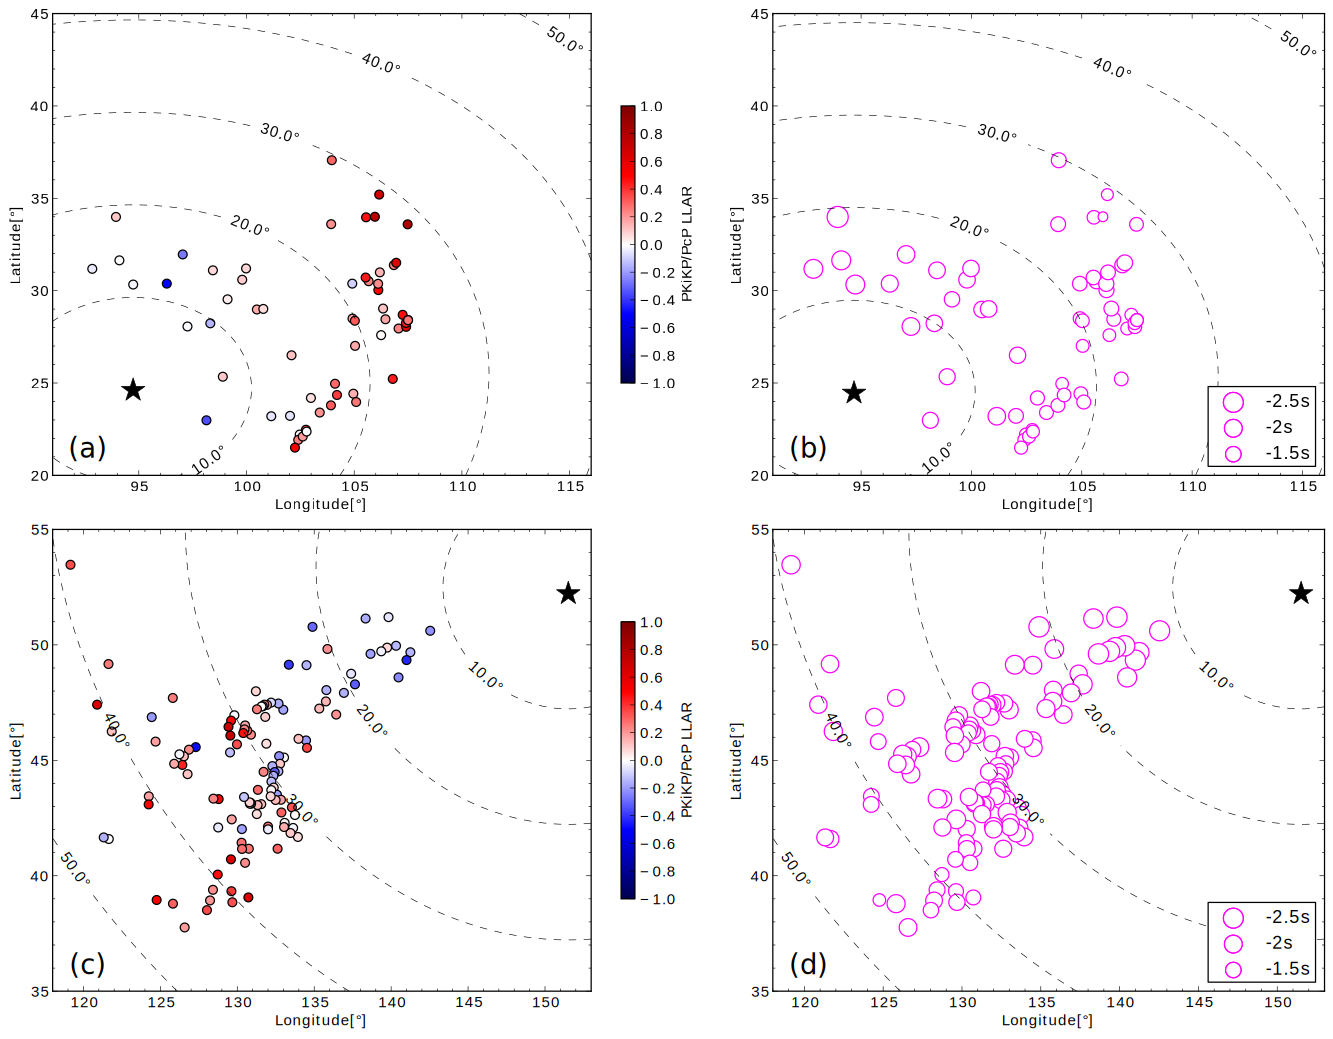
\includegraphics[width=\linewidth]{fig/chap4/bp_amp_res}
\caption{(a)、(b)事件2011/02/04(文中简称事件A)的PKiKP/PcP相对与PREM的对数振幅比残差和PKiKP-PcP走时残差分布;(c)、(d)对应事件2013/05/24(文中简称事件B)的结果,其余与(a)、(b)一致.图中的黑色五角星表示地震位置,等值线表示CMB上反射点对应的震中距位置.}
\label{fig:bp_amp_res}
\end{figure}

观察到的走时残差和LARR的正相关性和上一章所述及阿拉斯加Kenai半岛的情形一致,仅是尺度略微增大,因此也暗示了PKiKP/PcP振幅比受到了界面起伏变化的影响. 但这究竟是源于CMB的起伏还是类似\citet{Shen2016a}所提到的黄海周围ICB的界面起伏变化,还需要进一步讨论.

如前面提到的,对于事件A,在震中距10{\textdegree}到20{\textdegree}范围内观测的LARR
接近零,这就说明PREM就已经可以很好地拟合观测结果了. 因此,如果假定这部分区域的CMB和ICB的波速与密度
变化是PREM所描述的,而且该LARR“正常”区域的2秒走时残差负异常可以认为是中国下方背景外核厚度与PREM的
偏差,那么其东侧的LARR正异常和1~1.5秒的走时残差负异常就可以被认为是外核厚度的加厚,可能是CMB的局部
隆升造成的PcP振幅减弱或者是ICB的局部下沉造成的PKiKP振幅放大(图\ref{fig:model}). 假设是ICB的地
形下陷,那么这里的观测就要求ICB至少存在横向尺度为200km的起伏变化,但之前没有任何研究揭示ICB存在这样
的起伏尺度,而且就此事件而言,观测数量而言PKiKP要远远多于PcP,且超过40{\textdegree}震中距仍然有
清晰PKiKP的观测,这显示在大范围内ICB是稳定的、变化较平缓的. 对界面起伏来说,有下陷就必然有隆升,但就
本研究数据采样范围内,没有发现超过30{\textdegree}震中距出现增大的负走时残差;类似地,对于事件B,CMB上140{\textdegree}E,50{\textdegree}N附近可能存在一个平缓的局部下陷,因为此处的
走时残差相比负2秒的背景偏差还要低0.5秒左右,且存在普遍微负的LARR. 对应震中距30{\textdegree}附近
的反射点,又再次集中出现负的LARR,周围伴有正的LARR,而走时残差却并无增大,这可能说明在大范围隆升的CMB上还耦合了凹陷的地形.

除了界面起伏对观测结果的贡献,仍然需要考虑CMB和ICB的波速、密度等参数变化. 首先讨论CMB的速度异常. 若CMB上存在ULVZ,会增大LARR,而存在高速结构则有相反的效果. 根据~\citet{Thorne2004a,Xu2009a}的观测,本研究区域并CMB上不存在ULVZ,即使存在低速和高速的变化,对走时残差的影响也应和观测的结果截然相反,
因此这里可以排除CMB速度变化的影响. 其次,若考虑ICB的速度异常,要产生观测到的LARR,则必然要求ICB存
在数十km级别的速度扰动. 由于内核S波波速很难约束,这里近讨论P波波速. 根据之前采用PKIKP研究内核顶部
速度的研究~\citep{Tanak2012,Iritani2014},内核准东西半球P波速度分别较标准模型的变化均在1\%以内,即小于0.1km/s的变化,这种级别的变化是不可能造成明显的观测差异的~\citep{Koper2004a}. 最后,ICB密度差变化似乎能对LARR产生显著的影响,比如~\citet{Shen2016a}就用从ICB北到南0.6$g/cm^3$的密度差增加来解释LARR的增大. 然而这种解释看似合理,但基于本研究的观测,ICB密度变化不能解释走时残差和LARR的相关性,而且中国下方的ICB恰好位于前人定义的准东西半球~\citep{Tanaka1997}的正中,前人的地球动力学对流模型均认为内核东西半球存在不均匀的结晶环境. 准半球出现高衰减的和其上方ICB处于熔融状态存在关系,而西半球处于结晶冷凝状态,因而较为致密,且衰减较小~\citep{Tkalcic2015}. 同时很多研究都支持内核东半球的晶体粒度要更大~\citep{Niu2002,Iritani2014a},这样就更加减小了是由于ICB内外密度差增大造成PKiKP放大从而产生大的LARR的可能性. 综合以上的分析讨论,本研究认为中国下方CMB起伏变化是造成LARR和PKiKP-PcP走时残差区域变化的主要原因.

\section{对重复地震的PcP/PKiKP观测}

综合之前所有的结果,PcP和PKiKP的振幅比观测比往往存在很多不确定性,而这也是造成观测数据离散的一个很重
要的原因. 虽然利用IMS台阵可以对振幅比的观测质量作一个大致的评估,但对于单台观测要作一个这样的估计就很
难了. 这一节将利用相同台站对震源位置、深度和震源机制都很接近的两个地震的PKiKP和PcP记录来分析造
成单台站观测不确定性的因素,同时这也可以对振幅比和走时残差的观测结果作一定程度上的检验.


\begin{table}[ht]\xwu%
\centering
\begin{tabular}{*{11}{|c}|}
\hline
\diagbox[height=1cm,width=1.3cm,innerwidth=1cm]{}{事件} & \multicolumn{5}{c|}{2009/09/03 19:51:05, MW5.9, 104km} & \multicolumn{5}{c|}{2011/02/04 13:53:44, MW6.3, 116km}\\
\cline{1-11}
台站& $\Delta$({\textdegree}) & $\delta$t(s) & LARR & SNR${}_{PcP}$ & SNR${}_{PKiKP}$ & $\Delta$({\textdegree})  & $\delta$t(s) & LARR & SNR${}_{PcP}$ & SNR${}_{PKiKP}$ \\
\hline
GOM & 11.8502 & -2.26 & 0.033 & 2.916 & 2.548 & 11.5609 & -2.27 & -0.019 & 3.566 & 5.035\\
\hline
SGT & 14.9752 & -1.82 & 0.110 & 2.583 & 3.078 & 14.6917 & -1.78 & 0.076 & 3.928 & 2.980 \\
\hline
GTA & 15.6692 & -2.00 & -0.083 & 3.901 & 4.105 & 15.3762 & -1.97 & -0.260 & 5.995 & 2.535 \\
\hline
XIT & 23.0573 & -1.36 & 0.594 & 2.667 & 2.829 & 22.8458 & -1.36 & 0.447 & 5.134 & 5.546 \\
\hline
JUN & 23.5845 & -1.49 & 0.4306 & 4.607 & 3.883 & 23.3827 & -1.49 & 0.2239 & 6.225 & 9.314 \\
\hline
\end{tabular}
\caption{五个台站对两个距离仅30km地震的观测结果对比,包括PKiKP/PcP对数振幅比残差,相对PREM的走时残差以及每个震相的信噪比. 每个台站的PcP和PKiKP的信噪比均大于2.5,且每一道记录的中的PcP和PKiKP相关系数都在0.9之上.}
\label{repeat_obs}
\end{table}

选取的两个地震分别为上一节中2013年的事件和2009年9月3日距这个该事件发生处30km的另一个震级较小的地震,两个地震具体参数见表\ref{repeat_obs}. 根据Havard CMT解,这两个地震的震源机制基本是一样的,有
趣的是,这两个地震还有相反的震源时间函数,它们的P、PcP和PKiKP信号恰好是相反的. 2009年事件的震级较小,仅产生一百多个可见的PKiKP记录,经过信噪比、相关系数等筛选,最终得到同时记录到两个事件产生的PKiKP和PcP信号的五个台站(表\ref{repeat_obs},图\ref{fig:doublet_m}). 虽然这两个地震的近似程度不及之前内核差异旋转研究中用到
的地震对~\citep{Zhang2005},但它们在CMB上的反射点距离不足一个PcP波长(约13km),在ICB上的空间差
异则更小,因此这里也称这两个地震为“重复地震”. \citet{Tkalcic2013}总结了之前内核外核差异旋转的结
果,认为这种差异旋转是不稳定的,有时候会出现内外核相对静止的状态. 因此这里不考虑内核的这种运动,即使考虑每年0.5{\textdegree}的内核差异旋转速度,由于这两个地震发生时间间隔也仅有一年多,内核也只能转过10km左右,因此本研究认为认为两个地震几乎采样到相同位置的ICB和CMB.

\begin{figure}[ht]
\centering
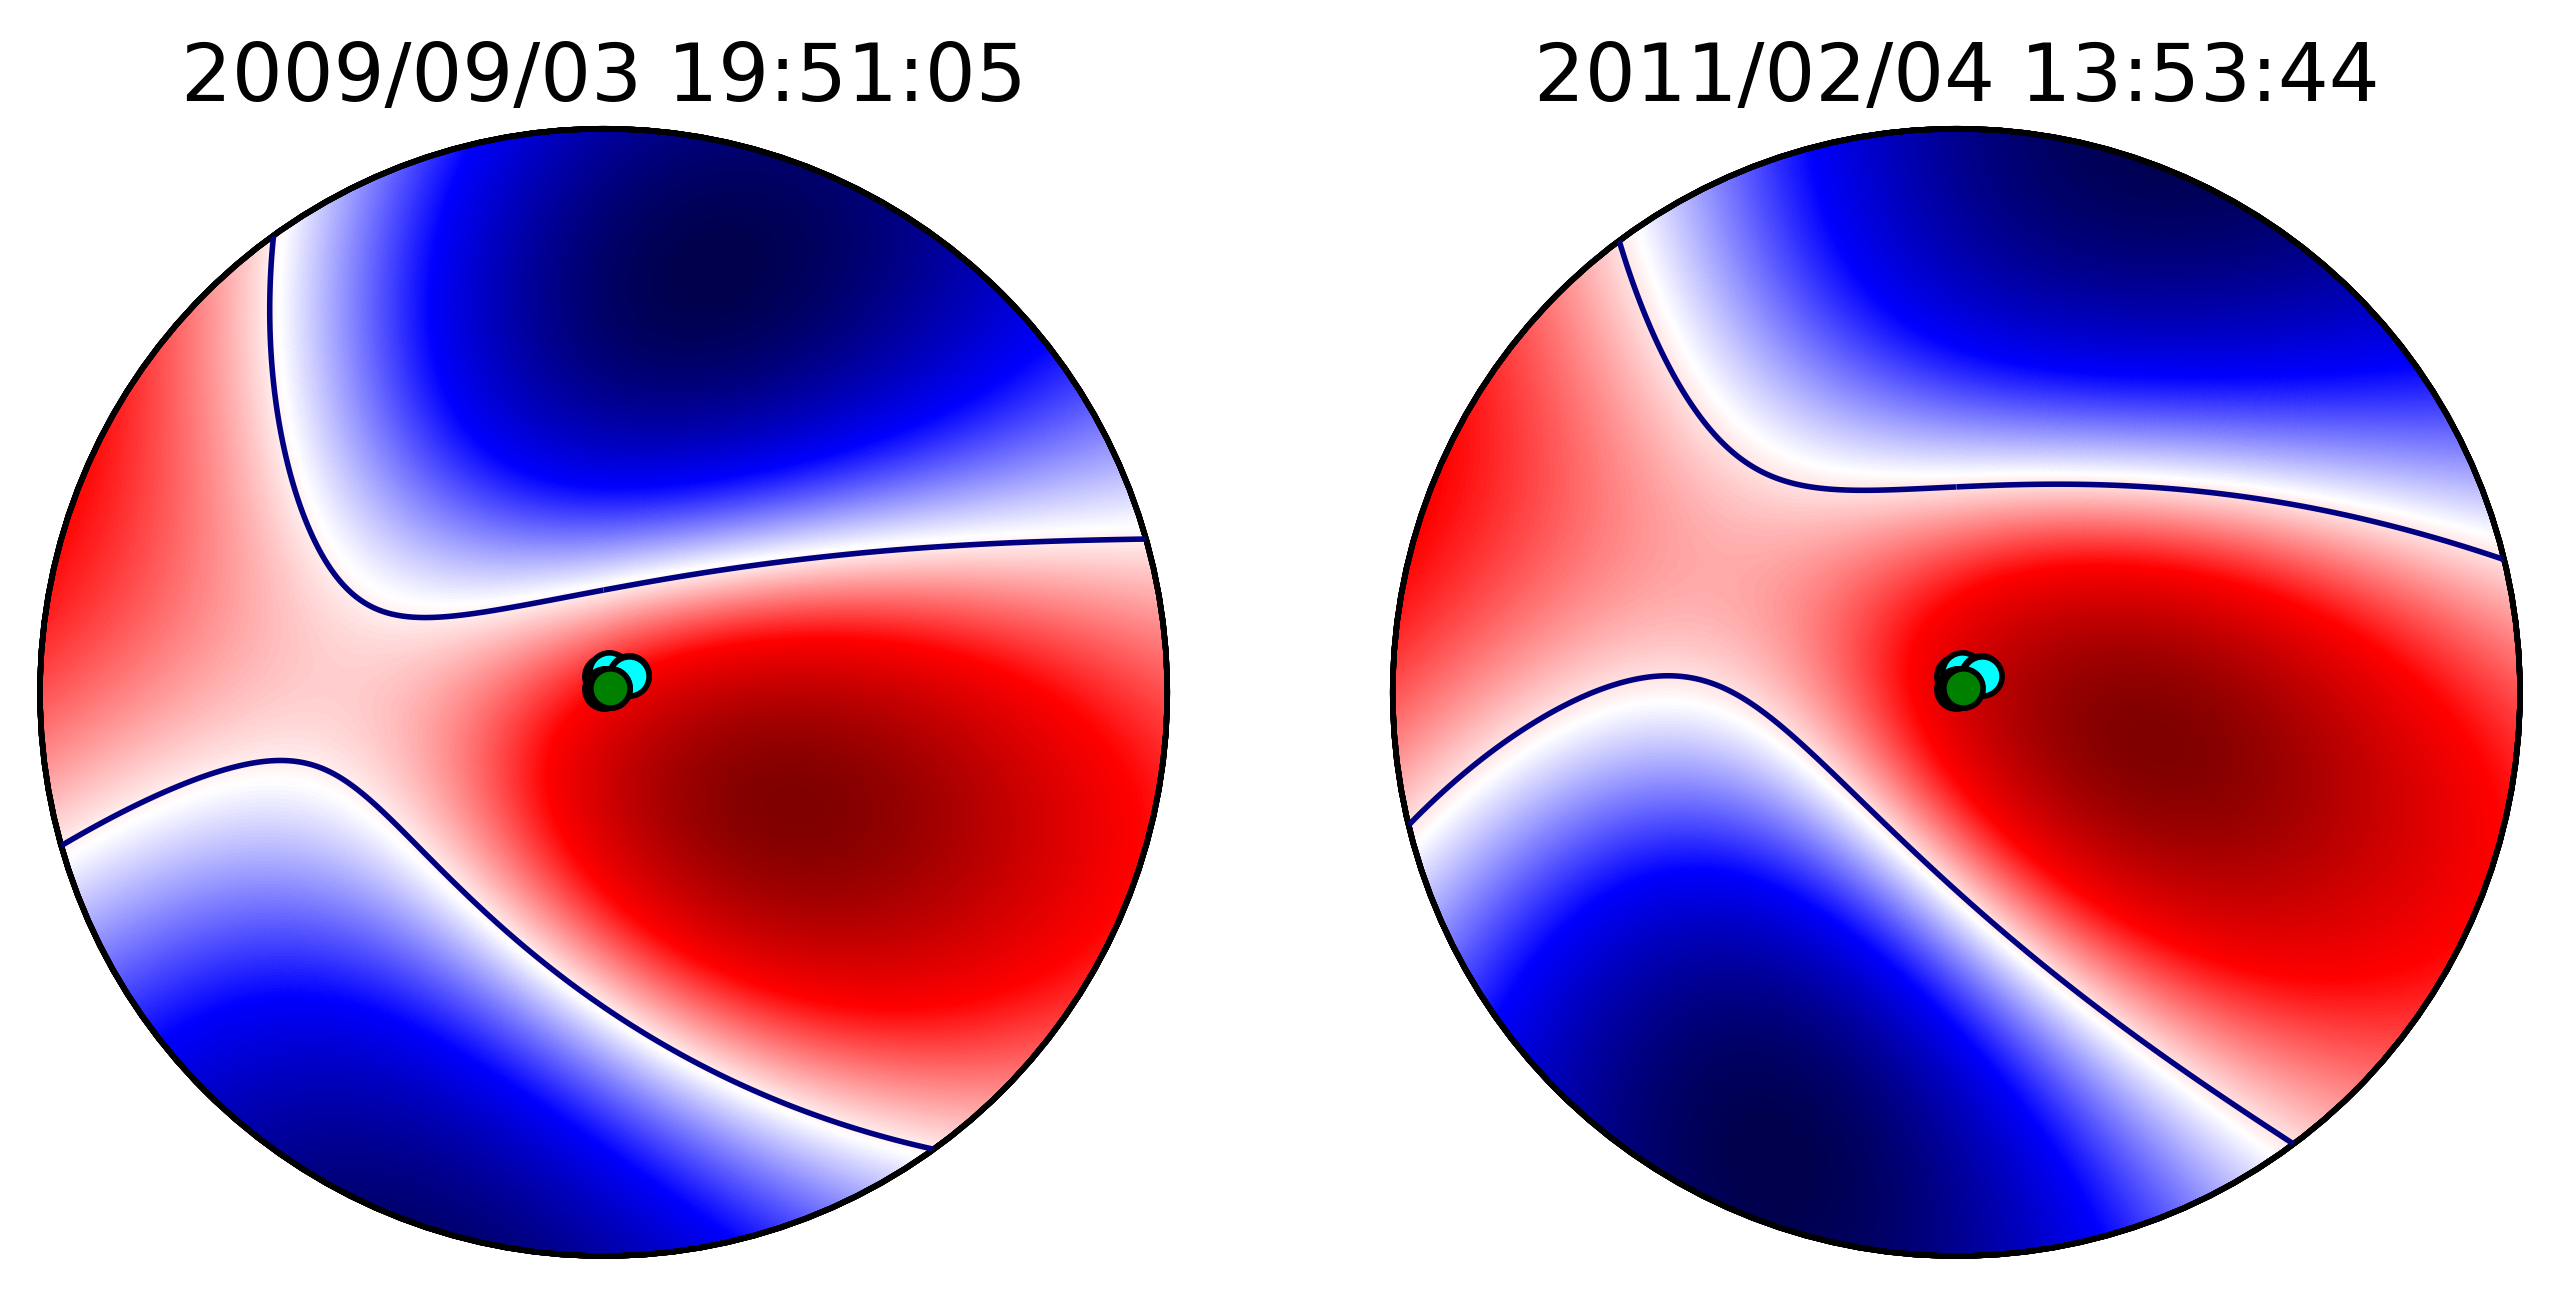
\includegraphics[width=0.68\linewidth]{fig/chap4/mt.png}
\caption{表\ref{repeat_obs}中两个地震的震源机制,浅蓝色圆圈对应PcP的出射位置,绿色圆圈对应PKiKP的出射位置.}
\label{fig:mt}
\end{figure}

\begin{figure}[ht]
\centering
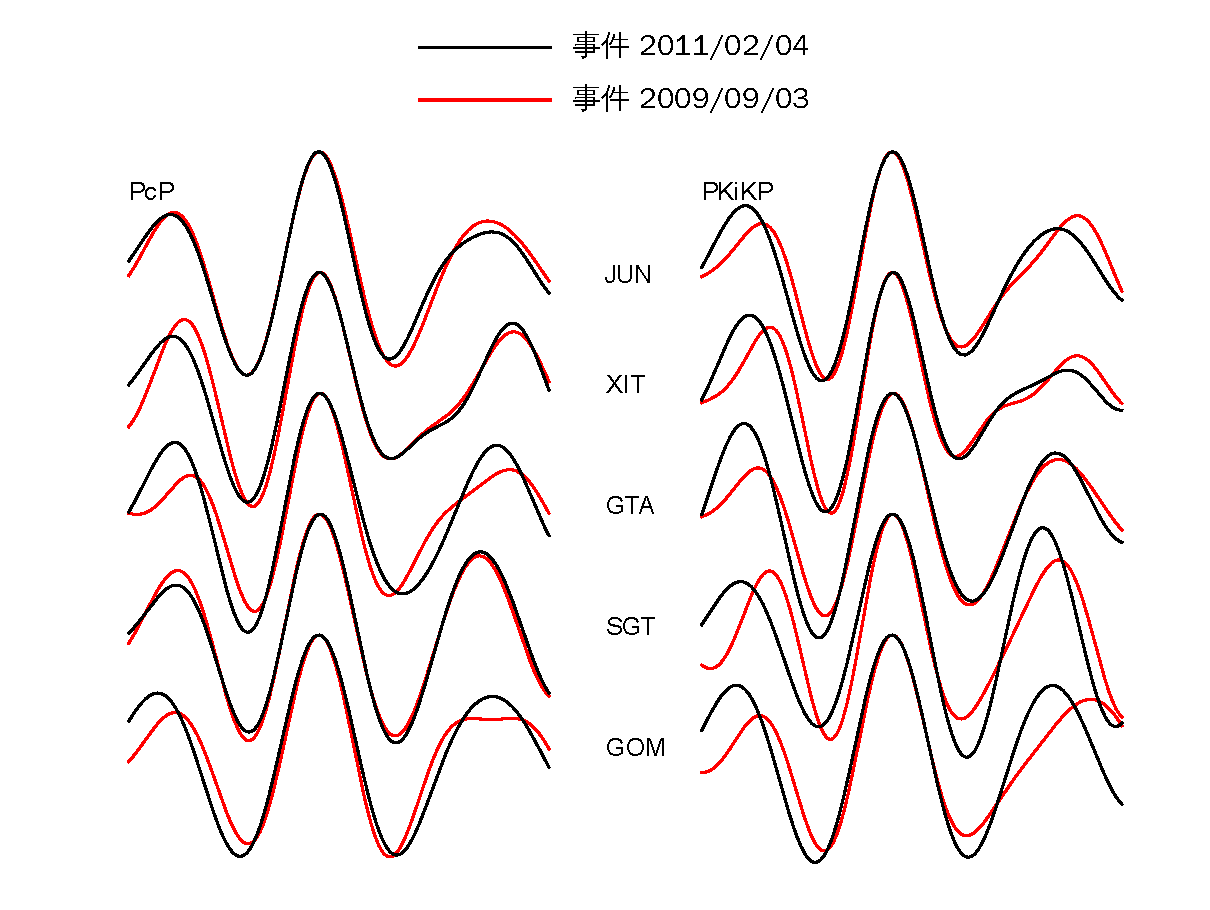
\includegraphics[width=0.8\linewidth]{fig/chap4/doublet_m}
\caption{表\ref{repeat_obs}中五个台站对两个地震的PcP和PKiKP记录,红色表示2009年的事件的波形,黑线表示2011年事件的波形. 对于2009年的事件,PcP和PKiKP的波形均做了倒转.}
\label{fig:doublet_m}
\end{figure}

通过比较同一个台站的两次记录,2009年地震的PKiKP/PcP对数振幅残差整体比2011年稍大,但差异也不是特别
显著,即两个地震的LARR同时接近零或同时偏大,这也说明对2011年地震PKiKP/PcP振幅比的观测还是比较可靠
的. 相比振幅观测的不稳定性,两个事件的PKiKP-PcP走时残差的观测则相当一致,单个台站的差别最多也只达到
几个采样间隔,这也体现出即使内核存在差异旋转,CMB和ICB也不存在可观测到的随时间变化的界面起伏变化. 因此这里认
为,造成单台站振幅比观测不稳定的因素主要有两个:(1)台站的信噪比;(2)地震的震级. 关于震级会影响PKiKP/PcP振幅比的观测结果,之前并没有研究提到过. 因为不论是CMB还是ICB,它们都不是理想的线弹性介质,反射波的振幅与入射波能量的大小也并不一定是线性关系,这也体现出使用PKiKP/PcP振幅比来约束CMB或者ICB结构方法上的缺陷.